\documentclass[tikz,border=0pt]{standalone}
\usetikzlibrary{calc}
% Palette: the 3D gym's colours (crates/core/src/mesh.rs, data/shaders/scene.frag).
\definecolor{sky}{HTML}{DCE6EE}
\definecolor{skyhi}{HTML}{F2F6F9}
\definecolor{wall}{HTML}{EDE6D3}
\definecolor{walldark}{HTML}{D6CCB4}
\definecolor{stripeblue}{HTML}{2F5CBF}
\definecolor{stripegold}{HTML}{F8C537}
\definecolor{window}{HTML}{CFE6FF}
\definecolor{windowlit}{HTML}{F6FBFF}
\definecolor{wood}{HTML}{DBA86B}
\definecolor{wooddark}{HTML}{B98549}
\definecolor{woodline}{HTML}{C9965A}
\definecolor{mat}{HTML}{2961CC}
\definecolor{matlit}{HTML}{4A82E8}
\definecolor{matdark}{HTML}{1C4597}
\definecolor{matseam}{HTML}{16377A}
\definecolor{red}{HTML}{DD3D38}
\definecolor{redlit}{HTML}{F06A5E}
\definecolor{reddark}{HTML}{A92A27}
\definecolor{yellow}{HTML}{F9C02E}
\definecolor{yellowlit}{HTML}{FFDB6B}
\definecolor{yellowdark}{HTML}{C9961C}
\definecolor{green}{HTML}{3FA866}
\definecolor{greenlit}{HTML}{62C98A}
\definecolor{greendark}{HTML}{2C7D4B}
\definecolor{pink}{HTML}{F27A93}
\definecolor{pinklit}{HTML}{F7A1B3}
\definecolor{orange}{HTML}{F28A2E}
\definecolor{orangelit}{HTML}{F7AE66}
\definecolor{orangedark}{HTML}{C2671A}
\definecolor{sky2}{HTML}{7FB8F0}
\definecolor{purple}{HTML}{8B5CC8}
\definecolor{skin}{HTML}{F2C49A}
\definecolor{skinlit}{HTML}{F8D8B8}
\definecolor{skindark}{HTML}{D9A47A}
\definecolor{skinb}{HTML}{B9835A}
\definecolor{skinbdark}{HTML}{93653F}
\definecolor{shirt}{HTML}{E2463F}
\definecolor{shirtdark}{HTML}{B23430}
\definecolor{shirtb}{HTML}{2F7DD8}
\definecolor{shirtbdark}{HTML}{225DA6}
\definecolor{shorts}{HTML}{21305A}
\definecolor{shortsdark}{HTML}{151F3D}
\definecolor{shoe}{HTML}{FFFFFF}
\definecolor{shoedark}{HTML}{D8DDE3}
\definecolor{hair}{HTML}{4A2F1C}
\definecolor{band}{HTML}{F8C537}
\definecolor{chick}{HTML}{FBE48F}
\definecolor{chicklit}{HTML}{FFF2BE}
\definecolor{chickdark}{HTML}{DCC064}
\definecolor{comb}{HTML}{E2302E}
\definecolor{beak}{HTML}{F28A2E}
\definecolor{noodle}{HTML}{57D163}
\definecolor{noodledark}{HTML}{3A9E45}
\definecolor{ball}{HTML}{D8302B}
\definecolor{balldark}{HTML}{A5211D}
\definecolor{balllit}{HTML}{F0645D}
\definecolor{duck}{HTML}{FFD12E}
\definecolor{duckdark}{HTML}{E0A814}
\definecolor{foam}{HTML}{2F6BE0}
\definecolor{foamdark}{HTML}{214FAD}
\definecolor{white}{HTML}{FFFFFF}
\definecolor{ink}{HTML}{1E2B45}
\definecolor{netline}{HTML}{9AA9BF}
\definecolor{glow}{HTML}{FFF4C2}
\begin{document}
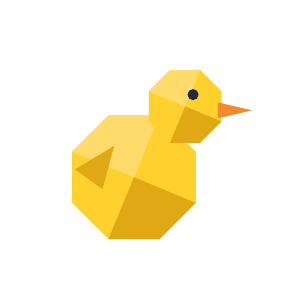
\begin{tikzpicture}[x=1cm,y=1cm]
\useasboundingbox (0,0) rectangle (3,3);
\fill[duck] (2.135,1.425) -- (1.675,1.885) -- (1.025,1.885) -- (0.565,1.425) -- (0.565,0.775) -- (1.025,0.315) -- (1.675,0.315) -- (2.135,0.775) -- cycle;
\fill[yellowlit] (1.35,1.1) -- (1.675,1.885) -- (1.025,1.885) -- (0.565,1.425) -- cycle;
\fill[duckdark] (1.35,1.1) -- (1.025,0.315) -- (1.675,0.315) -- (2.135,0.775) -- cycle;
\fill[duck] (2.462,2.191) -- (2.191,2.462) -- (1.809,2.462) -- (1.538,2.191) -- (1.538,1.809) -- (1.809,1.538) -- (2.191,1.538) -- (2.462,1.809) -- cycle;
\fill[yellowlit] (2,2) -- (2.191,2.462) -- (1.809,2.462) -- (1.538,2.191) -- cycle;
\fill[duckdark] (2,2) -- (1.809,1.538) -- (2.191,1.538) -- (2.462,1.809) -- cycle;
\fill[beak] (2.42,2.05) -- (2.85,1.95) -- (2.42,1.85) -- cycle;
\fill[ink] (2.1,2.15) circle (0.07);
\fill[duckdark] (0.6,1.2) -- (1.1,1.5) -- (0.95,0.95) -- cycle;
\end{tikzpicture}
\end{document}
